\chapter{2D CNN approach}
The very fist approach we tried was to develop from scratch a 2D CNN to recognize the violence in the videos, to do that we needed to extract the frame from the videos and feed it to the AI model since a 2D CNN process images.
\section{Frame extraction}
The idea initially was to do it with the help of \textit{FFpeg}. FFmpeg is a comprehensive software suite for recording, converting, and playing audio and video, it relies on libavcodec, a library for audio/video encoding. Following there is an example of usage.
\begin{lstlisting}[language=bash, caption={FFpeg example}, label={lst:FFpegExample}]
#!/bin/bash
# To force the frame rate of the output file to 24 fps:
$ ffmpeg -i input.avi -r 24 output.avi

\end{lstlisting}

Following there is the code used to extract the frames from the videos. For brevity we will show only the code used to extract the frames from the "fight" directory and the path are removed.
\begin{lstlisting}[language=bash, caption={Frame extraction}, label={lst:FrameExtraction}]

    !for f in $(ls [path_to_video]); do ffmpeg -i [path_to_video]/$f -vf fps=5 [path_to_frame]/${f%.*}-%03d.png; done;
\end{lstlisting}

This command uses FFmpeg to extract frames from a video file and save them as individual images, it iterates over each file in the specified directory and applies the FFmpeg command to convert the video to frames. The frames are saved with the same name as the original video file, followed by a three-digit number to indicate the frame sequence, the frames are saved in the specified output directory.
However, this method was found to not be flexible enough, in the light of new approach to the problem like a 3D CNN, more in the next chapter, so we decided to use a different approach, we decided extract the frames at runtime and feed them to the AI model with differences depending on the model and type of dataset fed to it. However this would have been to much of a workload, especially if we executed every time, so we decided to create a sort of cache made of pickle files \textit{.pkl}, this way we would have extracted the frames only once and then we would have loaded them. The following code shows the basic idea of the frame extraction process:

\begin{lstlisting}[language=python, caption={Pickles generation}, label={lst:PicklesGeneration}]
    # Function to load a dataset of videos with corresponding labels
   function load_video_dataset(dataset_path, pkl_config, create_on_missing):
        # Initialize empty lists for training and testing data and labels
        train_data = []
        train_labels = []
        test_data = []
        test_labels = []
    
        # Generate paths for storing pickle files
        pickles_dir =  f'{ROOT_PATH}/pickles'
        pickle_name = sha256([pickle key information])
    
        # Create a list of pickle file paths
        # f'{pickles_dir}/{pickle_name}-train_data.pkl'
        # f'{pickles_dir}/{pickle_name}-train_labels.pkl'
        # f'{pickles_dir}/{pickle_name}-test_data.pkl'
        # f'{pickles_dir}/{pickle_name}-test_labels.pkl'
        try:
            # Attempt to load data and labels from pickle files
            load_data_from_pickles([pickle_file_paths...])
    
        except FileNotFoundError:
            if create_on_missing:
                # Create a list of labeled video paths from the dataset
                labelled_paths = get_labeled_video_paths(dataset_path)
    
                # Shuffle the list of labeled video paths
                # Avoid deleting always the same videos at balancing time
                shuffle(labelled_video_paths)
    
                # Load and preprocess videos,balancing
                # the number of samples for each class
                labelled_frame = balance(labelled_paths, pkl_config)
    
                # Split the data into training and testing sets
                split_data(labelled_frame, pkl_config, min_amount)
    
                # Save the data and labels as pickle files
                save_pickles([pickle_file_paths...])
    
                # Update the pickle register with 
                #the new pickle file information
                update_pickle_register(pickles_dir, pickle_name, pkl_config)
    
        except Exception as e:
            print(f"An unexpected error occurred: {e}")
    
        # Return the loaded or newly created data and labels
        return train_data, train_labels, test_data, test_labels
    

\end{lstlisting}
The main idea is to create a 4 pickle files for each configuration (train\_data, train\_label, test\_data, test\_label), the pickle files are created only if they are not present, this way we can load them at runtime and avoid the frame extraction process. In case of creation needed, the frames are shuffled and then balanced, this is done to avoid deleting always the same videos. This process allows us not only to create pickles for 2D CNN but also for 3D CNN.

\section{Dataset cleaning}
As previously stated the dataset was very dirty, this problem would be a constant problem throughout the project, the dataset was composed of videos of different length, different resolution and different frame rate, in addition many videos contained black bars on the sides making any AI model learn from that instead of the actual features. To solve this problem we decided to crop the videos remove the black bars, this was done with the following code:

\begin{lstlisting}[language=Python, caption={Image Cropper}, label={lst:ImageCropper}]
    def crop(image, y_nonzero, x_nonzero):
    # If y_nonzero and x_nonzero are not provided, calculate them from the grayscale version of the image
    if y_nonzero is None or x_nonzero is None:
        gray_image = cv2.cvtColor(image, cv2.COLOR_BGR2GRAY)
        y_nonzero, x_nonzero = np.where(gray_image > 1)

    # Crop the image based on the calculated non-zero values
    cropped_image = image[np.min(y_nonzero):np.max(y_nonzero), np.min(x_nonzero):np.max(x_nonzero)]

    # Return the cropped image along with updated y_nonzero and x_nonzero values
    return cropped_image, y_nonzero, x_nonzero
\end{lstlisting}

However this proved to be not enough, the dataset was still very dirty, some videos contained writing on the screen, others were phone recording of desktop monitors. Ideally we could crop the videos in a square shape starting from the center, but this would cause a too big of a loss of information. The best solution would be to have bounding boxes for each video, but alas this was not the case and to manually made it would have been too much of a workload.

\section{First model}
For the first model we decided to use a 2D CNN, the model was composed of 2 convolutional layers, 2 max pooling layers and 2 fully connected layers, the model was trained for 30 epochs with a batch size of 32, patient 15, the optimizer used was Adam. This parameters were found to be the best from early experimentation runs. The model was trained on the dataset with the black bars removed, the dataset was composed of 2 classes, violence and no-violence, the model was trained on 80\% of the dataset and tested on the remaining 20\%, the validation set was 30\% of the training set with a hold out methodology.  

\begin{figure}[]
    \centering
    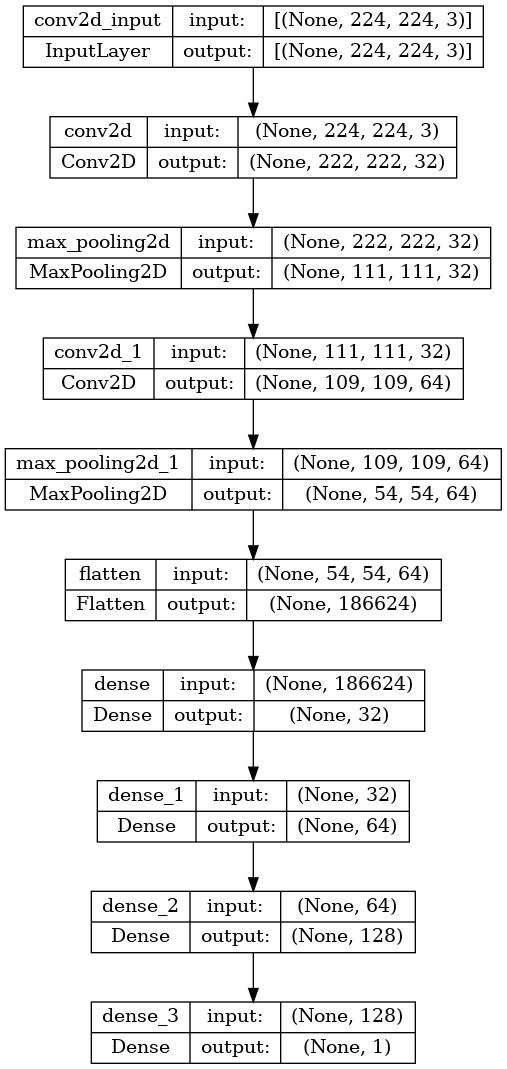
\includegraphics[width=0.8\textwidth, height=1.3\textwidth]{images/2D_3_noDrop.png}
    \caption{Initial 2D CNN model}
    \label{fig:First2DCNN}
\end{figure}

\begin{figure}[]
    \centering
    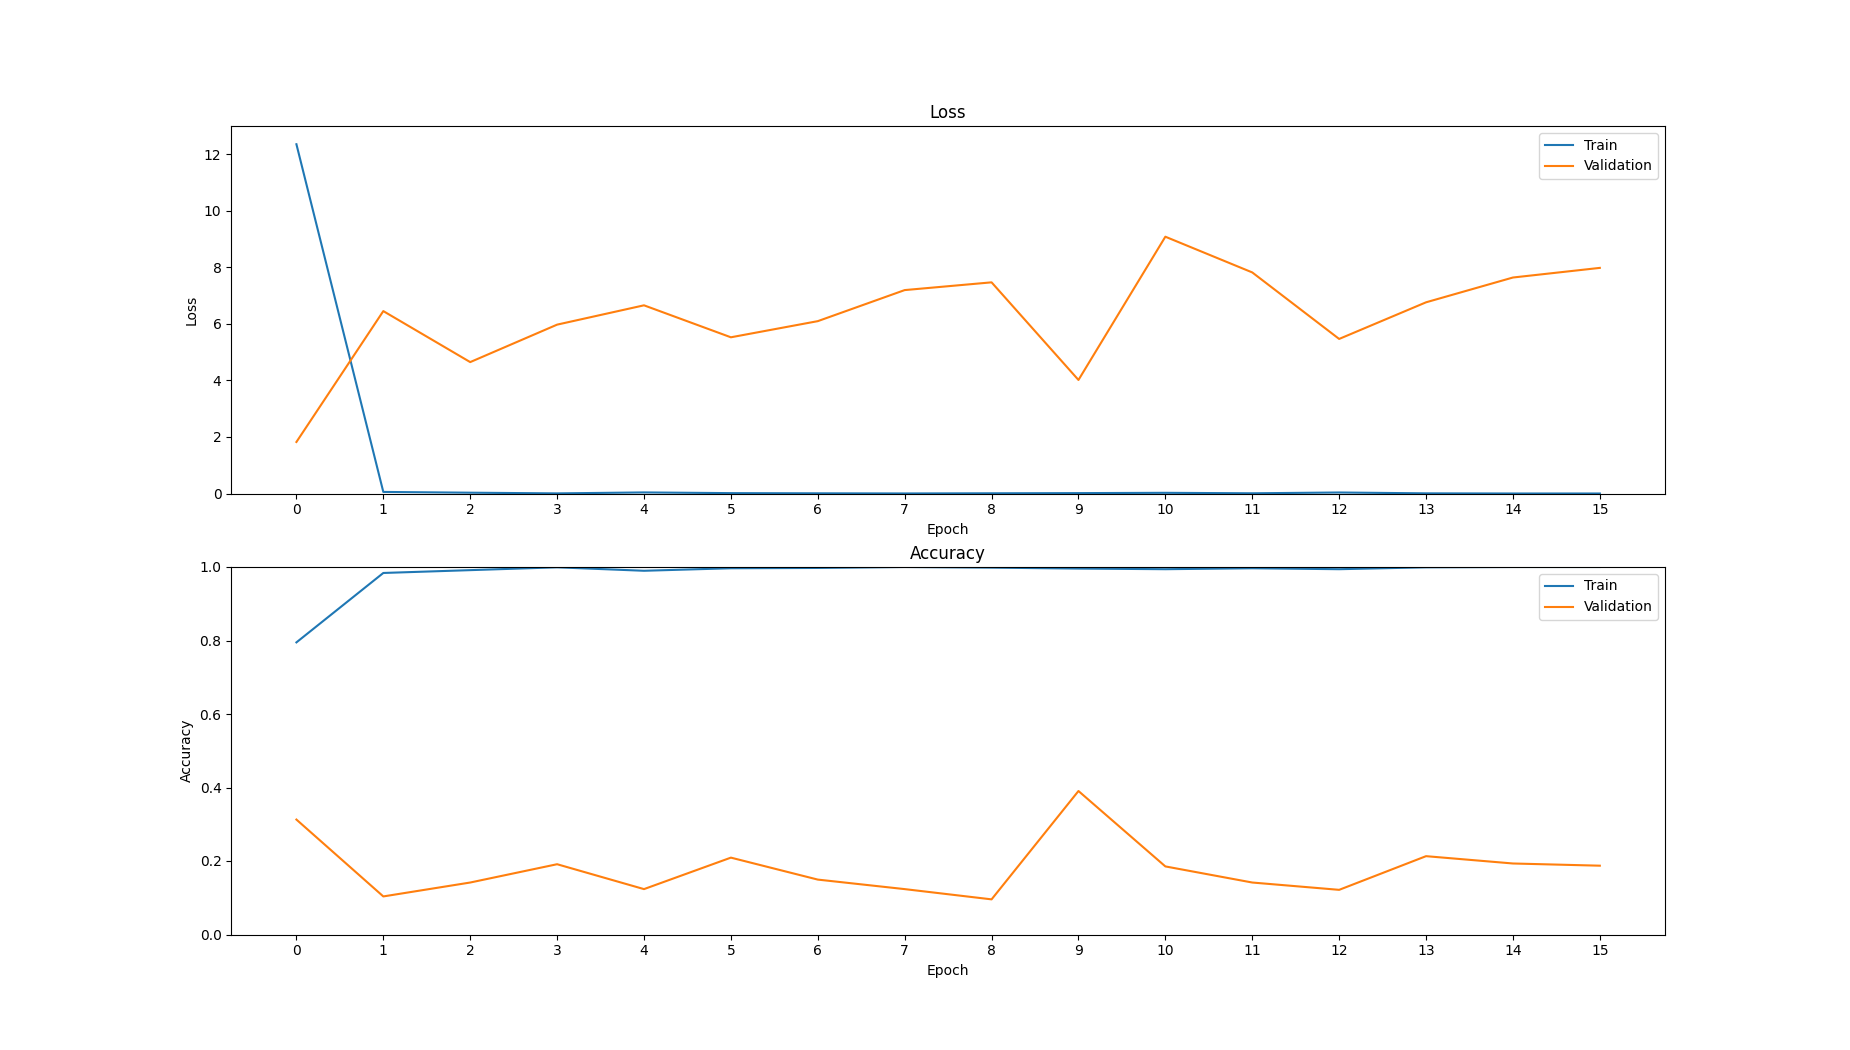
\includegraphics[width=1\textwidth]{images/731a-2D3-86ad-history.png}
    \caption{Training history of the first model}
    \label{fig:First2DCNNHistory}
\end{figure}

\begin{figure}[]
    \centering
    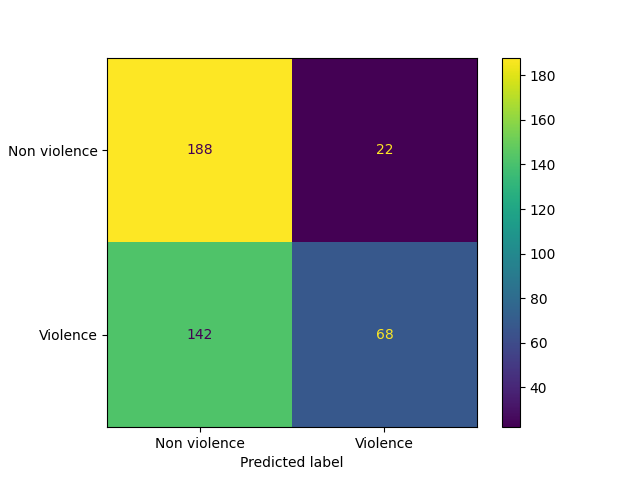
\includegraphics[width=0.8\textwidth]{images/731a-2D3-86ad-conf_matrix.png}
    \caption{Confusion matrix of the first model}
    \label{fig:First2DCNNConfusionMatrix}
\end{figure}


The first comment to be made is that the confusion matrix is heavily bias towards the \textit{Non violence} side. This is due to the fact that the dataset can be quite chaotic and the model is not able to learn the features of the videos. For example the model may learn form the Non violence part of the dataset that gatherings of people are not to be flagged as violence, however this could easily lead to false positive (Violence images classified as Non violence ones).

Another comment is to be made regarding the validation loss and accuracy which is quite unstable and unsatisfactory, this could signal overfitting and general failing in extrapolating the main features of the videos.
\pagebreak
\section{Second model}
For the second model we decided to amp the convolution layers to 3 as shown in Fig. \ref{fig:Second2DCNN}, other parameters remained unchanged this was done to see if the model would have been able to learn more features from the videos. 
We decided to use a cautious approach since the problem presented itself as a very complicated one and we did not want to aport to many changes in a single \textit{pass} to avoid a time consuming trial and error process. As can be seen in Tab. \ref{tab:2DConfront} the second model performed better than the first one by a small margin, but alas the confusion matrix is more balanced in respect to the first one, this could indicate a better generalization capability. Speaking of generalization capability, the validation loss and accuracy are still quite unstable and unsatisfactory as shown in Fig. \ref*{fig:Second2DCNNHistory}, so this must be addressed in the next models.
\begin{table}[H]
    \centering
    \resizebox{\textwidth}{!}{%
    \begin{tabular}{c|ccc|ccc|}
    \cline{2-7}
                                                & \multicolumn{3}{c|}{\textbf{FIRST MODEL}}                                                          & \multicolumn{3}{c|}{\textbf{SECOND MODEL}}                                                         \\ \cline{2-7} 
                                                & \multicolumn{1}{c|}{\textbf{PRECISION}} & \multicolumn{1}{c|}{\textbf{RECALL}} & \textbf{F1-SCORE} & \multicolumn{1}{c|}{\textbf{PRECISION}} & \multicolumn{1}{c|}{\textbf{RECALL}} & \textbf{F1-SCORE} \\ \hline
    \multicolumn{1}{|c|}{\textbf{ACCURACY}}     & \multicolumn{1}{c|}{}                   & \multicolumn{1}{c|}{}                & \textbf{0.60952}  & \multicolumn{1}{c|}{}                   & \multicolumn{1}{c|}{}                & \textbf{0.62381}  \\ \hline
    \multicolumn{1}{|c|}{\textbf{MACRO AVG}}    & \multicolumn{1}{c|}{0.66163}            & \multicolumn{1}{c|}{0.60952}         & 0.57481           & \multicolumn{1}{c|}{0.62494}            & \multicolumn{1}{c|}{0.62381}         & 0.62295           \\ \hline
    \multicolumn{1}{|c|}{\textbf{WEIGHTED AVG}} & \multicolumn{1}{c|}{0.66263}            & \multicolumn{1}{c|}{0.60952}         & 0.57481           & \multicolumn{1}{c|}{0.62494}            & \multicolumn{1}{c|}{0.62381}         & 0.62295           \\ \hline
    \end{tabular}%
    }
    \caption{Confront between the two models}
    \label{tab:2DConfront}
    \end{table}

\begin{figure}[]
    \centering
    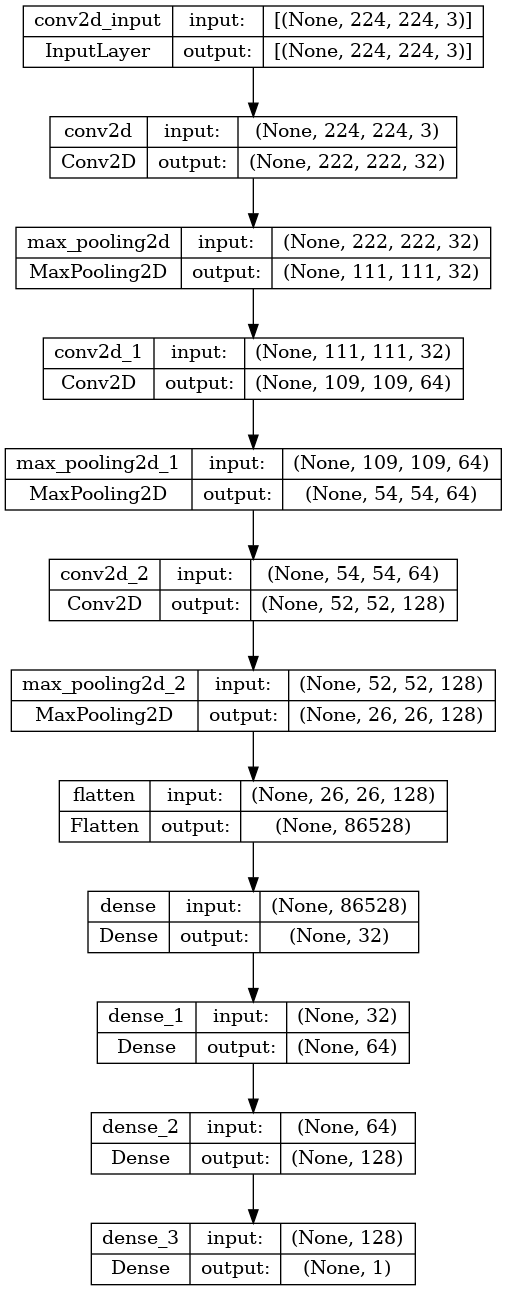
\includegraphics[width=0.8\textwidth, height=1.3\textwidth]{images/2D_35_noDrop.png}
    \caption{Second 2D CNN model}
    \label{fig:Second2DCNN}
\end{figure}


\begin{figure}[]
    \centering
    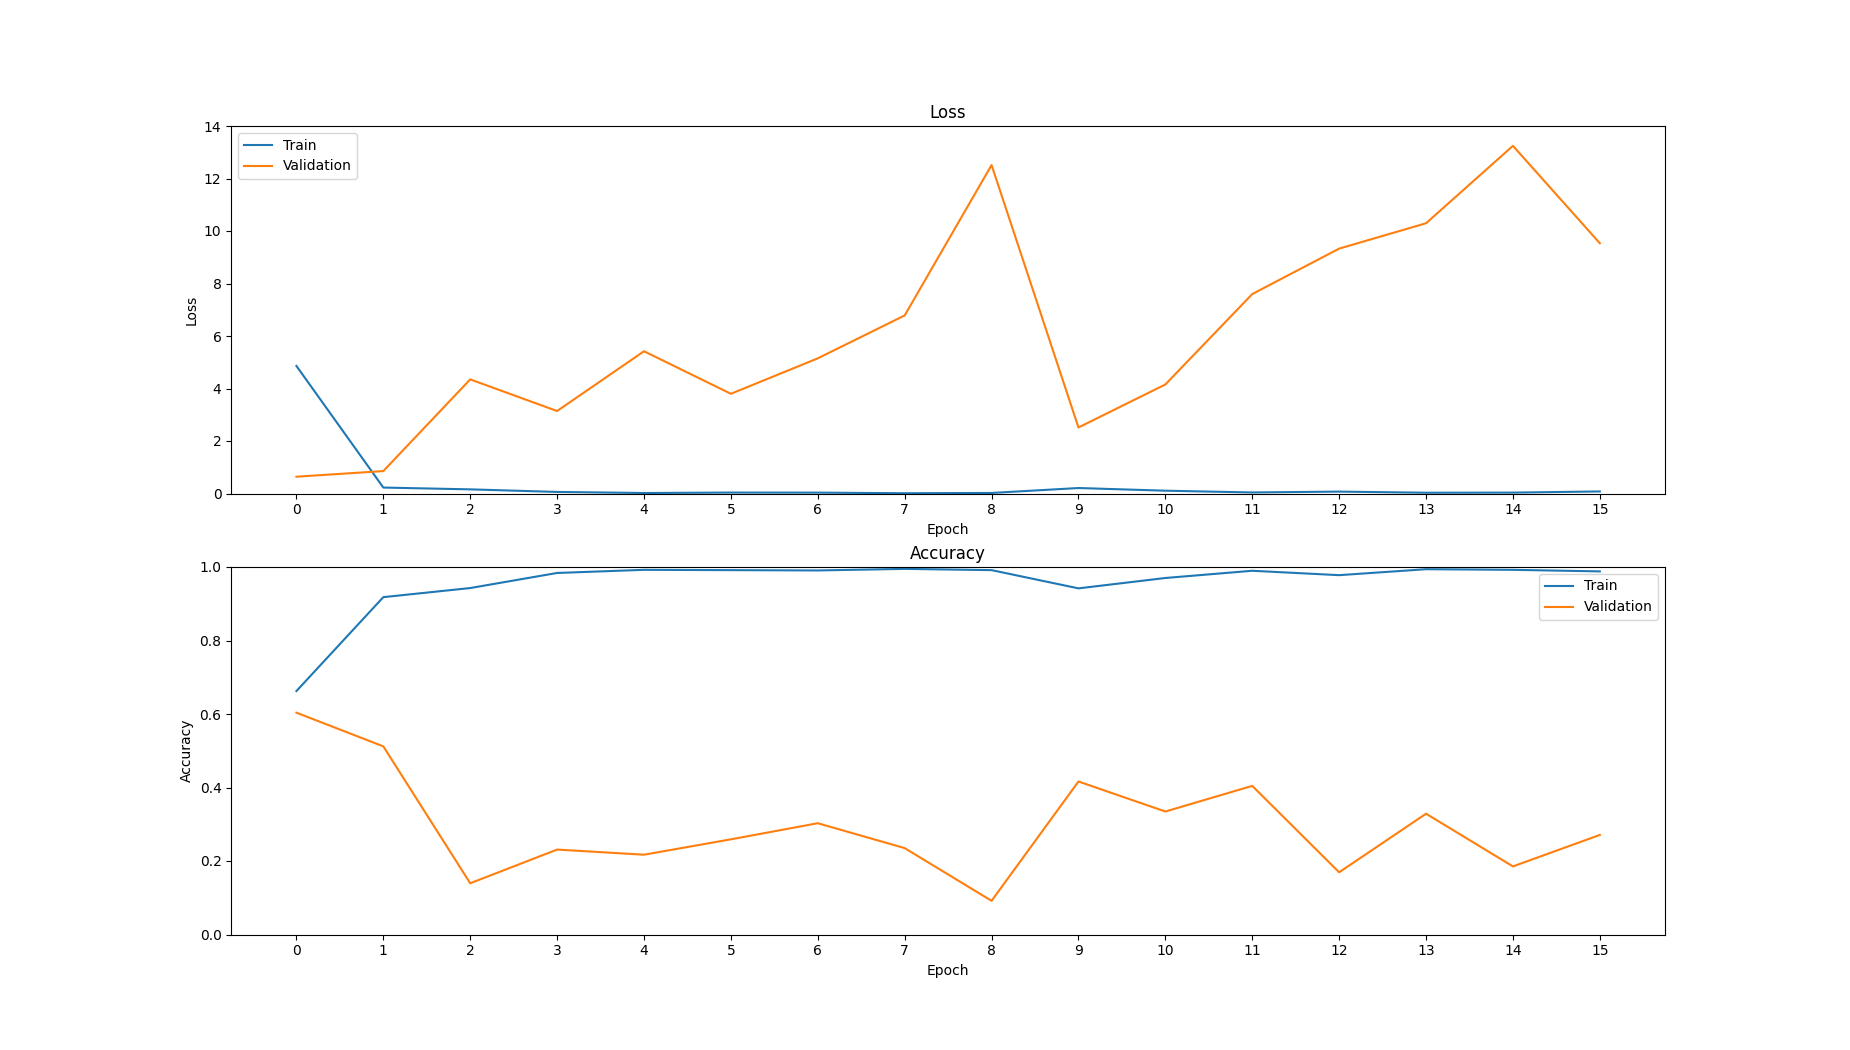
\includegraphics[width=1\textwidth]{images/731a-2D35-86ad-history.png}
    \caption{Training history of the second model}
    \label{fig:Second2DCNNHistory}
\end{figure}


\begin{figure}[]
    \centering
    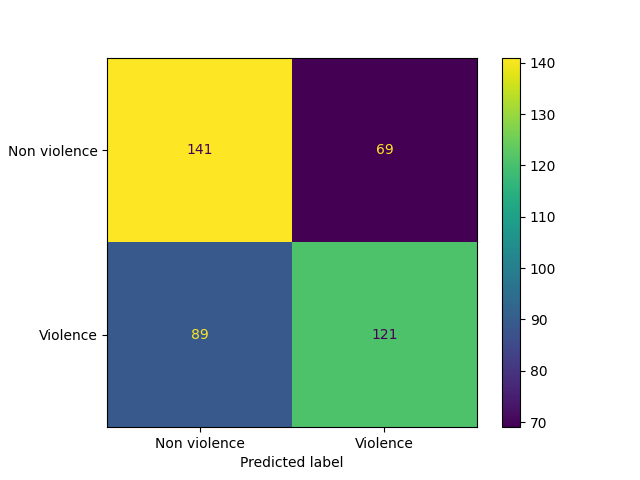
\includegraphics[width=0.8\textwidth]{images/731a-2D35-86ad-conf_matrix.png}
    \caption{Confusion matrix of the second model}
    \label{fig:Second2DCNNMatrix}
\end{figure}

\pagebreak
\section{Addressing the generalization problem}
As previously stated the generalization problem was a constant one, to addressed this we decide to add dropout layers in the model, we also decided to, according to common practice, decrease the number of dense layers. The other parameters remained unchanged. Unfortunately this did not solve the problem as shown in Fig. \ref{fig:Third2DCNNHistory} and Fig. \ref{fig:Third2DCNNMatrix}, the model is still not able to generalize well, this could be due to the fact that the dataset is too small and too dirty or the problem could be too hard to solve with a \textit{simple} 2D CNN, to achieve a better solution we would have needed a bigger dataset, but this was not available to us.
\begin{figure}[]
    \centering
    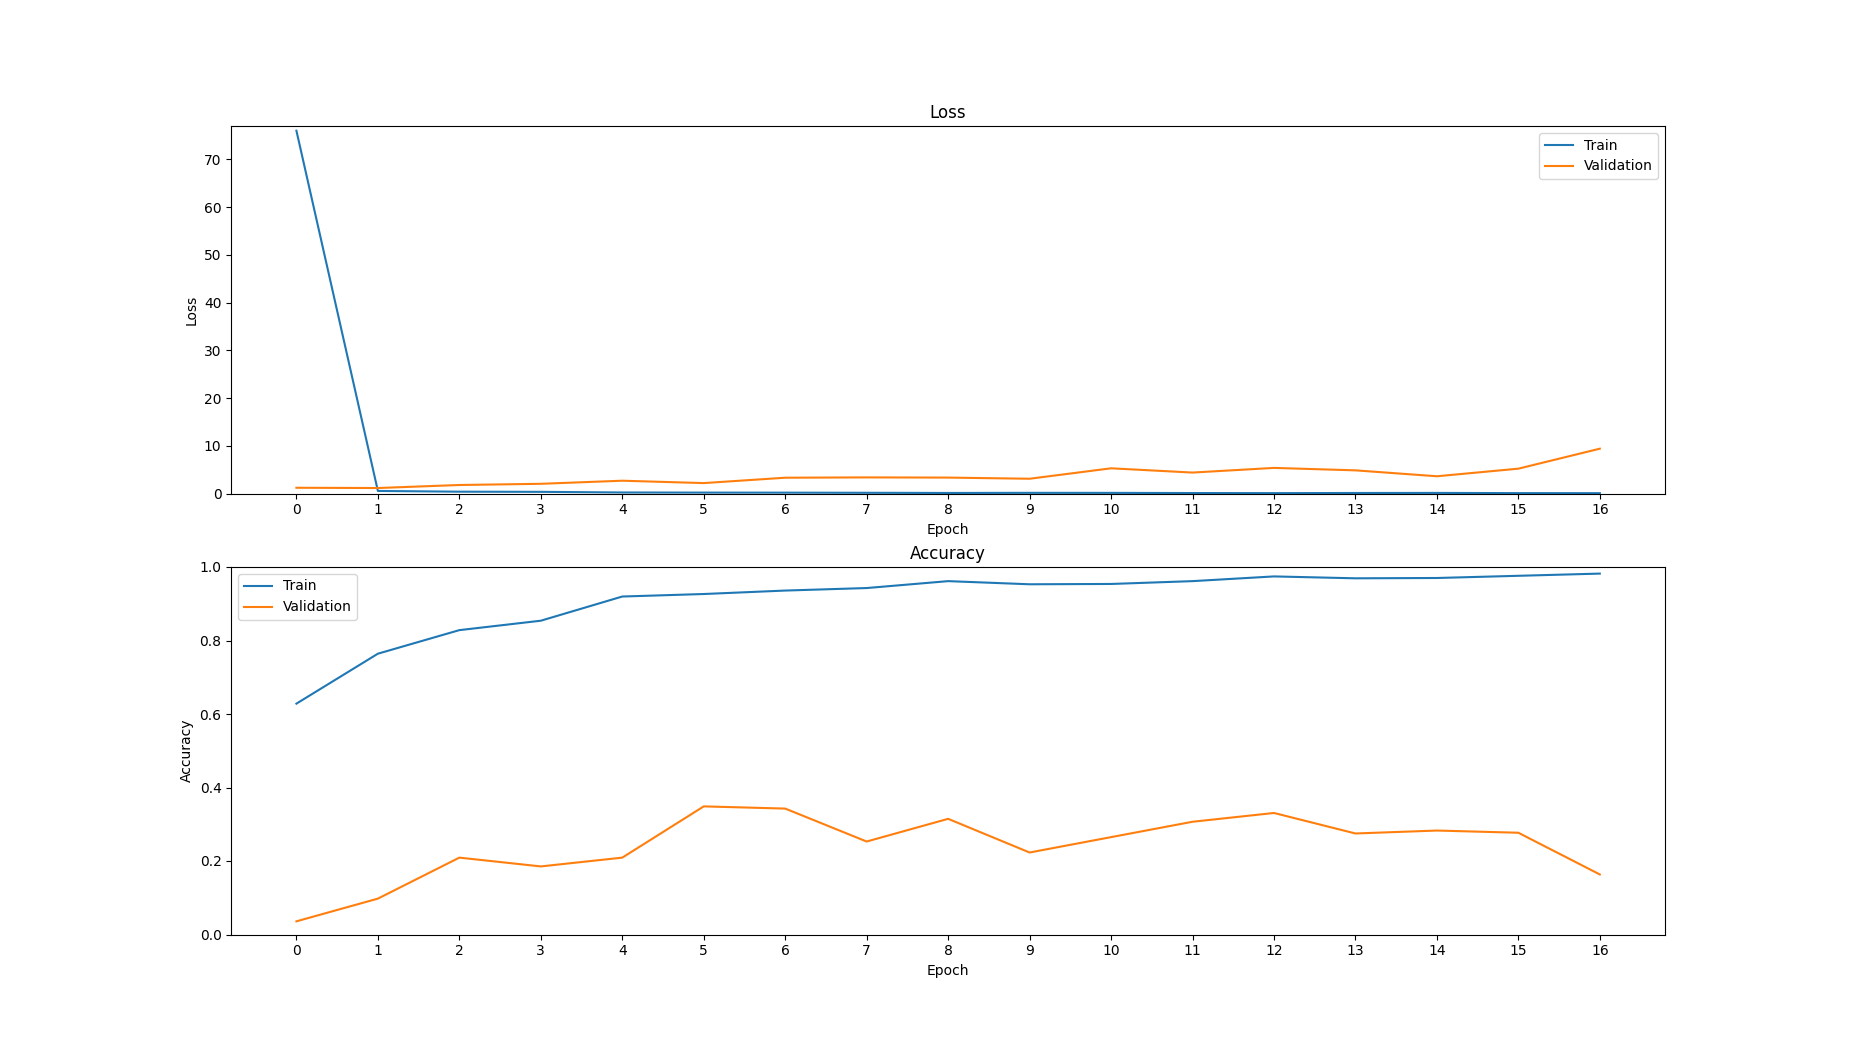
\includegraphics[width=1\textwidth]{images/731a-2DFabioFinal-86ad-history.png}
    \caption{Training history of the third model}
    \label{fig:Third2DCNNHistory}
\end{figure}
\begin{figure}[]
    \centering
    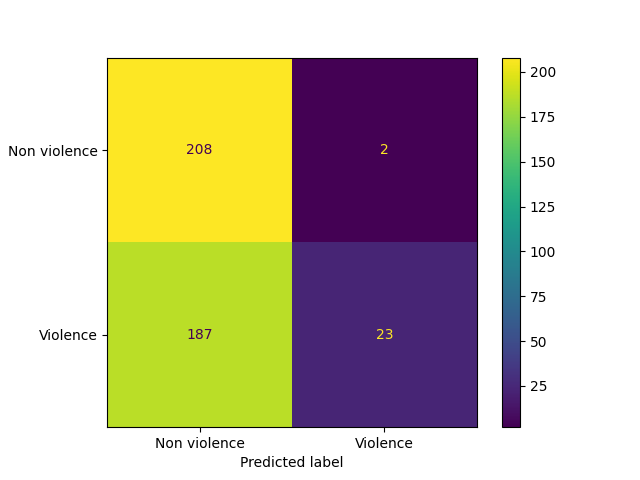
\includegraphics[width=0.8\textwidth]{images/731a-2DFabioFinal-86ad-conf_matrix.png}
    \caption{Confusion matrix of the third model}
    \label{fig:Third2DCNNMatrix}
\end{figure}

\section{Pretrained models}
Since the 2D CNN approach was not working we decided to try a different approach, we decided to use pretrained models.
TO BE CONTINUED
